\documentclass[11pt]{scrartcl}

\usepackage[utf8]{inputenc}

\usepackage[T1]{fontenc}
\usepackage[french]{babel}

\usepackage{textcomp}
\usepackage{amsmath}
\usepackage{amssymb}
\usepackage{mathtools}
\usepackage{siunitx}
\usepackage{lmodern}
\usepackage{graphicx}
\usepackage{tabularx}

\usepackage{microtype}
\usepackage[parfill]{parskip}
\usepackage[hidelinks]{hyperref}

\title{Vie artificielle}
\subtitle{Automates cellulaires}

\author{Lieselotte \textsc{Marchal}}

\begin{document}
    \maketitle
    
    \section{Blob}
        \subsection{Modélisation du monde}
            Le monde est constitué de texels à trois composantes :
            \begin{itemize}
                \item Un booléen indiquant si la case est occupée par un agent ;
                \item Un réel indiquant l'orientation d'un tel agent ;
                \item Un réel indiquant le taux de matériel présent sur la case.
            \end{itemize}
        
        \subsection{Règles de simulation}
            À chaque pas de temps, les agents sont d'abord déplacés de \texttt{STEP\_LENGTH}.
            Plusieurs agents allants sur la même case sont combinés en un seul agent ; le type de combinaison est déterminée par l'option \texttt{BOUNCE}.
            
            Le matériel est ensuite diffusé uniformément sur un côté de \texttt{DIFFUSION\_SIZE}, puis évaporée selon \texttt{RETENTION\_RATE}.
            
            Les agents déposent enfin \texttt{DEPOSIT\_AMOUNT} matériel sur chaque case dans un carré de côté \texttt{DEPOSIT\_SIZE}, puis se réorientent
            selon les paramètres \texttt{SENSOR\_DISTANCE}, \texttt{SENSOR\_SIZE} et \texttt{SENSOR\_ANGLE}.
        
        \subsection{Propriétés}
            Du fait que certains agents se combinent en un seul, l'automate n'est pas réversible.
            Comme des agents ne sont jamais recréés, la densité de l'automate est décroissante et tend vers une constante positive.
        
        \subsection{Simulation}
            Les figures~\ref{fig:phy-rgb} et \ref{fig:phy-hsv} montrent une simulation à $t = 5000$ qui converge en un vaisseau spatial allant
            indéfiniment à droite.
            
            \begin{figure}[h]
                \centering
                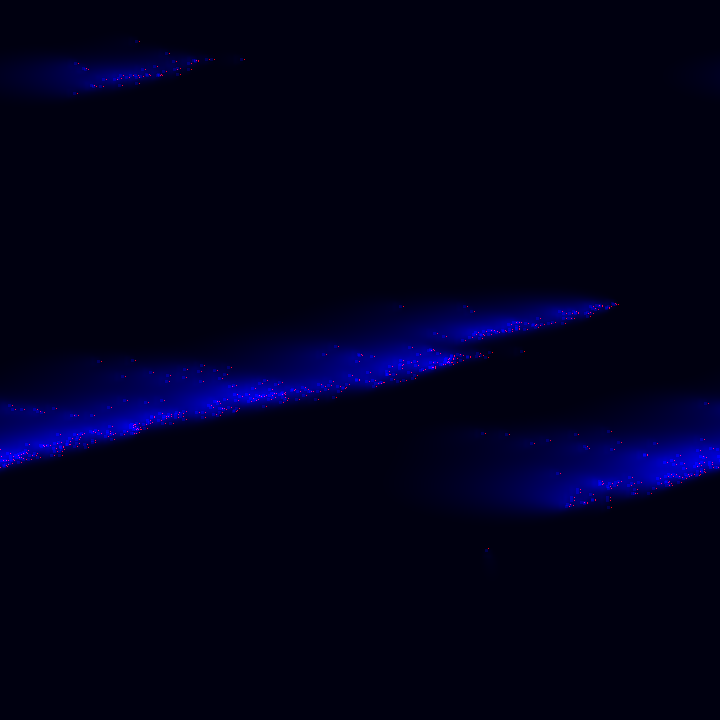
\includegraphics[width=\textwidth]{physarum_rgb}
                \caption{Blob ; en bleu la concentration de matériel, en rouge les agents.}\label{fig:phy-rgb}
            \end{figure}
            
            \begin{figure}[h]
                \centering
                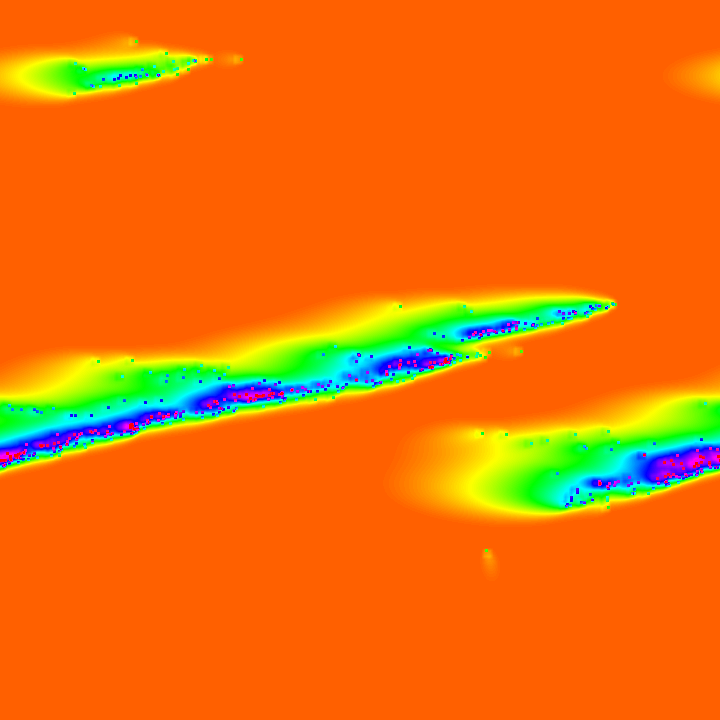
\includegraphics[width=\textwidth]{physarum_hsv}
                \caption{Blob ; concentration de matériel. Les agents viennent d'émettre et sont ainsi visibles.}\label{fig:phy-hsv}
            \end{figure}
    
\end{document}

